\documentclass[ignorenonframetext, professionalfonts, hyperref={pdftex, unicode}]{beamer}

\usetheme{Copenhagen}
\usecolortheme{wolverine}

%Packages to be included
%\usepackage{graphicx}

\usepackage[russian]{babel}
\usepackage[utf8]{inputenc}
\usepackage[T1]{fontenc}

%%\usepackage[orientation=landscape, size=custom, width=16, height=9.75, scale=0.5]{beamerposter}

\usepackage{textcomp}

\usepackage{beamerthemesplit}

\usepackage{ulem}

\usepackage{verbatim}

\usepackage{ucs}


\usepackage{listings}
\lstloadlanguages{bash}

\lstset{escapechar=`,
	extendedchars=false,
	language=sh,
	frame=single,
	tabsize=2, 
	columns=fullflexible, 
%	basicstyle=\scriptsize,
	keywordstyle=\color{blue}, 
	commentstyle=\itshape\color{brown},
%	identifierstyle=\ttfamily, 
	stringstyle=\mdseries\color{green}, 
	showstringspaces=false, 
	numbers=left, 
	numberstyle=\tiny, 
	breaklines=true, 
	inputencoding=utf8,
	keepspaces=true,
	morekeywords={u\_short, u\_char, u\_long, in\_addr}
	}

\definecolor{darkgreen}{cmyk}{0.7, 0, 1, 0.5}

\lstdefinelanguage{diff}
{
    morekeywords={+, -},
    sensitive=false,
    morecomment=[l]{//},
    morecomment=[s]{/*}{*/},
    morecomment=[l][\color{darkgreen}]{+},
    morecomment=[l][\color{red}]{-},
    morestring=[b]",
}

\author[Epam]{{\bf Epam}\\Low Level Programming Department}

%\institution[EPAM]{EPAM}
%\logo{\includegraphics[width=1cm]{logo.png}}


\title{Введение в GNU/Linux}


%%%%%%%%%%%%%%%%%%%%%%%%%%%%%%%%%%%%%%%%%%%%%%%%%
%%%%%%%%%% Begin Document  %%%%%%%%%%%%%%%%%%%%%%
%%%%%%%%%%%%%%%%%%%%%%%%%%%%%%%%%%%%%%%%%%%%%%%%%




\begin{document}

\begin{frame}
	\frametitle{}
	\titlepage
	\vspace{-0.5cm}
	\begin{center}
	%\frontpagelogo
	\end{center}
\end{frame}


\begin{frame}
	\tableofcontents
	[hideallsubsections]
\end{frame}

\section{О курсах}

\mode<all>{\begin{frame}{Цель курса}
	\begin{center}
		\Huge
		Увеличение популярности GNU/Linux среди программистов.

		\hrulefill

		\normalsize
		Воспитание потенциальных сотрудников ;-)
	\end{center}
\end{frame}


\begin{frame}{Состав курса}
	\begin{itemize}
		\item Представление об архитектуре GNU/Linux дистрибутива
			\pause
		\item "Ежедневные" навыки работы в консоли
			\pause
		\item Языки программирования
			\begin{itemize}
					\item shell (Bash)
					\item Python
					\item C
			\end{itemize}
			\pause
		\item Работа с классическими средствами разработки для ОС Linux
			\pause
		\item Все, чего вы не знали и боялись спросить
	\end{itemize}
\end{frame}
}

\section*{GNU/Linux}

\begin{frame}{Основы ОС Linux}

	\begin{block}{Вопрос}
	Почему Linux является самой популярной
	свободной операционной системой?
	\end{block}

	\pause

	\begin{block}{Ответ}
	\begin{itemize}
		\item \textcopyleft -- Copyleft
		\item ``Философия'' Unix
		\item Открытые стандарты
	\end{itemize}
	\end{block}

\end{frame}


%%%%%%%%%%%%%%%%%%%%%%%%%%%%%%%%%%%%%%%%%   
%%%%%%%%%% Content starts here %%%%%%%%%%
%%%%%%%%%%%%%%%%%%%%%%%%%%%%%%%%%%%%%%%%%

\section[Принципы]{Базовые принципы ОС Linux}

\subsection{GNU/Linux}

\mode<all>{\input{../../slides/intro/vocabulary}}

\subsection{Лицензии}

\mode<all>{\begin{frame}{Авторское право и лицензии}

	\begin{block}{Авторское право}
		 Возникает по факту создания ПО 

		\begin{itemize}
			\item Неимущественные права
			\item Имущественные права
		\end{itemize}
	\end{block}

	\pause

	\begin{block}{Лицензии}
		Лицензия -- средство передать какие-либо права на продукт либо его часть.

		Необходима для защиты авторских прав. 
		Средство для возможности законно пресечь несанкционирование копирование,  использование или распространение ПО. 
	\end{block}
\end{frame}


\begin{frame}{Лицензии: открытые и свободные}
	\begin{block}{ Р.Столлман: 4 свободы}
		\begin{itemize}
			\item Свобода 0: Свобода запускать программу в любых целях.
			\item Свобода 1: Свобода изучения работы программы и адаптация её к вашим нуждам. 
				Доступ к исходным текстам является необходимым условием.
			\item Свобода 2: Свобода распространять копии,  так что вы можете помочь вашему товарищу.
			\item Свобода 3: Свобода улучшать программу и публиковать ваши улучшения,
				так что всё общество выиграет от этого.
				Доступ к исходным текстам является необходимым условием.
		\end{itemize}
	\end{block}
\end{frame}


\begin{frame}{Лицензии: permissive}
	\begin{columns}
	\column{0.3\textwidth}
		\center
\includegraphics[width=2cm,natwidth=144,natheight=144]{../../slides/intro/three-arrows@2x.png}

	\column{0.6\textwidth}

	\begin{itemize}
		\item BSD
		\item MIT
		\item Apache
	\end{itemize}
	\end{columns}

	\begin{block}{I want it simple and permissive.}
		\begin{itemize}
			\item практически не ограничивают свободу действий пользователей ПО и разработчиков, работающих с исходным кодом.
			\item По своему духу, распространение работы под пермиссивной лицензией схоже с помещением работы в общественное
				достояние, но не требует отказа от авторского права.
		\end{itemize}
	\end{block}

\end{frame}


\begin{frame}{\textcopyleft -- Copyleft}

	\begin{columns}
	\column{0.3\textwidth}
		\center
\includegraphics[width=2cm,natwidth=144,natheight=138]{../../slides/intro/circular@2x.png}

	\column{0.6\textwidth}

	\begin{itemize}
		\item GPL
		\item LGPL
		\item AGPL
	\end{itemize}
	\end{columns}


	\begin{block}{I care about sharing improvements.}
	
	Авторское лево -- концепция и практика использования законов авторского права для обеспечения 
	невозможности ограничить любому человеку право использовать,  изменять и распространять как 
	исходное произведение,  так и произведения,  производные от него.
	\end{block}


	При копилефте все производные произведения должны распространяться под той же лицензией,
	что и оригинальное произведение.

\end{frame}



}

%%\subsection{Принципы проектирования переносимых программ}

%%\mode<all>{\begin{frame}{Главные ориентиры}
	\begin{itemize}
		\item кроссплатформенная переносимость
		\item открытые стандарты
	\end{itemize}
\end{frame}

\begin{frame}{Немного цитат}
Дуг Макилрой, изобретатель каналов <<pipes>>, сформулировал несколько постулатов,применимых для разработки ПО:
\pause
	\begin{itemize}
		\item пишите программы,  которые выполняют одну функцию и делают это хорошо;
			\pause
		\item пишите программы,  которые будут работать вместе;
			\pause
		\item пишите программы,  поддерживающие текстовые потоки,  поскольку они являются универсальным интерфейсом.
	\end{itemize}

\end{frame}


\begin{frame}{"Философия" UNIX}
	это {\bfseries не} философия,  а общие рекомендации по проектированию ПО,  накопленные сообществом программистов на опыте десятилетий разработок программ,  которые взаимодействуют друг с другом.
\end{frame}

\begin{frame}{1. Правило модульности}
	\begin{block}{Следует писать простые части,  связанные ясными интерфейсами.}
Единственным способом создания сложной программы,  не обреченной заранее на провал,  является сдерживание ее глобальной сложности.
	\end{block}
Т.е. построение программы из простых частей, соединенных четко определенными интерфейсами, 
так что большинство проблем являются локальными, 
и тогда можно рассчитывать на обновление одной из частей без разрушения целого.
\end{frame}

\begin{frame}{Размер кода и ошибки}
	\begin{center}
		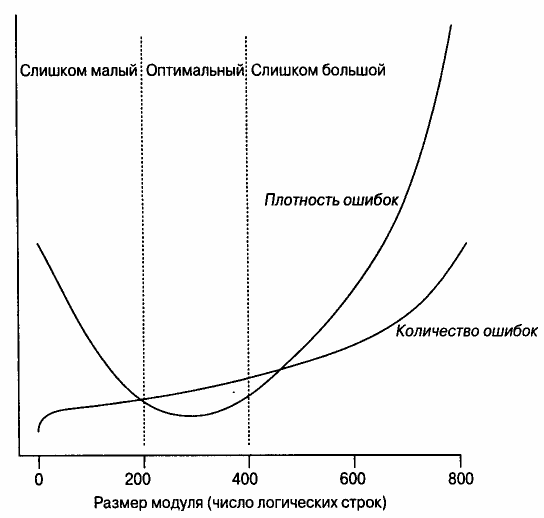
\includegraphics[width=200px]{../../slides/intro/errors_density-graph.png}
	\end{center}
\end{frame}

\begin{frame}{2. Правило ясности}
	\begin{block}{Ясность -- лучше чем мастерство.}
		Последующее обслуживание программы -- важная и дорогостоящая часть жизненного цикла программы.
	\end{block}
	\pause
Писать программы необходимо так,  как если бы вы знали,  что последующей поддержкой будет заниматься неуравновешенный псих с топором,  знающий ваш домашний адрес!
\end{frame}

\begin{frame}{3. Правило композиции}
	\begin{block}{Следует разрабатывать программы,  которые будут взаимодействовать с другими программами.}
		Если разрабатываемые программы не способны взаимодействовать друг с другом,  то очень трудно избежать создания сложных монолитных  программ.
	\end{block}
	Методы взаимодействия могут быть сильными и слабыми -- по возможности рекомендуется использовать слабые методы и текстовые форматы передачи данных.
\end{frame}

\begin{frame}{4. Правило разделения}
	\begin{block}{Следует отделять политику от механизма и интерфейсы от основных модулей (engine).}
		Примеры политики и механизма:\\
		вид GUI и операции отрисовки, клиент (front-end) -- сервер (back-end), сценарии и библиотеки и др.
	\end{block}
	При жесткой связи политики и механизма:
	\begin{itemize}
		\item политика становится негибкой и усложняется ее изменение;
		\item изменение политики имеет строгую тенденцию к дестабилизации механизмов.
	\end{itemize}
\end{frame}

\begin{frame}{5. Правило простоты}
	\begin{block}{Необходимо проектировать простые программы и <<добавлять сложность>> только там,  где это необходимо.}
	\end{block}
	Основные причины добавления сложности:
	\begin{itemize}
		\item человеческий фактор (часто -- желание <<выпендриться>>);
		\item проектные требования,  продиктованные текущей модой,  маркетингом или «левой пяткой заказчика»;
	\end{itemize}
\end{frame}

\begin{frame}{6. Правило расчетливости}
	\begin{block}{Пишите большие программы,  только если после демонстрации становится ясно,  что ничего другого не остается.}
		Под <<большими программами>> здесь понимаются программы с большим объемом кода и значительной внутренней сложностью.
	\end{block}
\end{frame}

\begin{frame}{7. Правило прозрачности}
	\begin{block}{Для того,  чтобы упростить проверку и отладку программы,  ее конструкция должна быть обозримой.}
		Программа {\itshape прозрачна}, если при ее минимальном изучении можно понять, что она делает и как.\\
		Программа {\itshape воспринимаема},  когда она имеет средства для мониторинга и отображения внутреннего состояния.
	\end{block}
	Необходимо использовать достаточно простые форматы входных и выходных данных.\\
	Интерфейс должен быть приспособлен для использования в отладочных сценариях.
\end{frame}

\begin{frame}{8. Правило устойчивости}
	\begin{block}{Устойчивость -- следствие	прозрачности и простоты.}
		Программа является {\itshape устойчивой},  когда она выполняет свои функции в неожиданных условиях,  которые выходят за рамки предположений разработчика,  как и в нормальных условиях.\\
		Программа является {\itshape простой},  если происходящее в ней не представляется сложным для восприятия человеком.
	\end{block}
	Один из способов организации -- модульность(простые блоки,  ясные интерфейсы)\\
	Следует избегать частных случаев!
\end{frame}

\begin{frame}{Пример неусточивого ПО}
	\begin{center}
		
\includegraphics[width=1\textwidth]{../../slides/intro/exploits_of_a_mom_rus.png}
	\end{center}
\end{frame}


\begin{frame}[fragile]{Пример <<простой>> программы}
	\begin{center}
		\begin{verbatim}
+++++++++++++++++++++++++++++++++++++++++++++
+++++++++++++++++++++++++++.+++++++++++++++++
++++++++++++.+++++++..+++.-------------------
---------------------------------------------
---------------.+++++++++++++++++++++++++++++
++++++++++++++++++++++++++.++++++++++++++++++
++++++.+++.------.--------.------------------
---------------------------------------------
----.-----------------------.
		\end{verbatim}
	\end{center}
\end{frame}

\begin{frame}{9. Правило представления}
	\begin{block}{Знания следует оставлять в данных,  чтобы логика программы могла быть примитивной и устойчивой.}
		Даже простую логику бывает сложно проверить,  но даже сложные структуры данных являются довольно простыми для моделирования и анализа (например диаграмма 50 узлов дерева и блок-схема 50 строк кода)
	\end{block}
	Если можно выбирать между усложнением структуры данных и усложнением кода,  то лучше выбирать первое.\\
	Примеры: ascii,  генератор html-таблицы.
\end{frame}

\begin{frame}{10. Правило наименьшего удивления}
	\begin{block}{При проектировании интерфейсов всегда следует использовать наименее неожиданные элементы.}
		Необходимо учитывать характер предполагаемой аудитории и традиции платформы.
	\end{block}
	Оборотная сторона: следует избегать создания внешне похожих вещей,  слегка отличающихся в действительности,  поскольку {\itshape кажущаяся привычность порождает ложные ожидания}.
\end{frame}

\begin{frame}{11. Правило тишины}
	\begin{block}{Если программе нечего сказать,  то пусть лучше молчит.}
		Внимание и сосредоточенность пользователя -- ценный и ограниченный ресурс,  который требуется только в случае необходимости.
	\end{block}
	Важная информация не должна смешиваться с подробными сведениями о работе программы.
\end{frame}

\begin{frame}{12. Правило восстановления}
	\begin{block}{Когда программа завершается аварийно,  это должно происходить явно (шумно) и по возможности быстро.}
		Если программа не способна справиться с ошибкой,  то необходимо завершить ее работу так,  чтобы максимально упростить диагностику.
	\end{block}
	Для сетевых служб следует следовать рекомендации Постела:\\
	<<{\itshape Будьте либеральны к тому,  что принимаете,  и консервативны к тому,  что отправляете}>>
\end{frame}

\begin{frame}{13. Правило экономии}
	\begin{block}{Время программиста дорого -- поэтому задача экономии его времени более приоритетна,  по сравнению с экономией машинного времени.}
		Компьютер железный -- ему не скучно (с) программистская мудрость
	\end{block}
	Использование высокоуровневых языков и <<обучение>> машины выполнять больше низкоуровневой работы по программированию,  что приводит к правилу 14.
\end{frame}

\begin{frame}{14. Правило генерации}
	\begin{block}{Избегайте кодирования вручную; если есть возможность -- пишите программы для создания программ.}
		Использование генераторов кода оправданно,  когда они могут повысить уровень абстракции,  
		т.е. когда язык спецификации для генератора проще,  чем сгенерированный код,  
		и код впоследствии не потребует ручной доработки.
	\end{block}
	Примеры: грамматические и лексические анализаторы,  генераторы make-файлов,  построители GUI-интерфейсов.
\end{frame}

\begin{frame}{15. Правило оптимизации}
	\begin{block}{Сначала -- опытный образец,  потом -- оптимизирование.}
		Добейтесь стабильной работы,  только потом оптимизируйте.
	\end{block}
	\begin{block}{Керниган и Плоджер:}
		90\% актуальной и реальной функциональности лучше,  чем 100\% функциональности перспективной и сомнительной
	\end{block}
	\begin{block}{Кнут:}
		преждевременная оптимизация -- корень всех зол
	\end{block}
	\begin{block}{Кент Бек (экстремальное программирование):}
		заставьте программу работать,  заставьте работать ее верно,  а затем сделайте ее быстрой
	\end{block}
\end{frame}

\begin{frame}{16. Правило разнообразия}
	\begin{block}{Не следует доверять утверждениям о <<единственно правильном пути>>.}
		Никто не обладает умом,  достаточым для оптимизации всего или для предвидения всех возможных вариантов использования создаваемой программы.
	\end{block}
\end{frame}

\begin{frame}{17. Правило расширяемости}
	\begin{block}{Разрабатывайте для будущего. Оно наступит быстрее,  чем вы думаете.}
		При проектировании протоколов или форматов файлов следует делать их самоописательными,  для того,  чтобы их можно было расширить.
	\end{block}
	{\itshape Всегда},  следует либо включать номер версии,  либо составлять формат из самодостаточных,  
	самоописательных команд так,  чтобы можно было легко добавить новые директивы,  
	а старые удалить, <<не сбивая с толку>> код чтения формата.
\end{frame}

\begin{frame}{Все правила сразу}
	\begin{center}
	{\Huge\bfseries K.I.S.S.}

	Keep It Simple,  Stupid!
	\end{center}
\end{frame}


}

\section{Дистрибутивы ОС Linux}

\mode<all>{\begin{frame}{Дистрибутив ОС GNU/Linux}
	\begin{block}{ Определение}
		\only<1>{\center{\bf{?}}}
		\pause
		\only<2->{Набор программного обеспечения на базе ядра Linux, распространяющийся как единое целое.}
	\end{block}
\end{frame}


\begin{frame}{Задачи дистрибутива}
	\begin{itemize}
		\item Предоставление комплекта ПО (ядро + утилиты)
		\item Средства установки и настройки
		\item Средства обновления
	\end{itemize}
\end{frame}

\begin{frame}{Различия между дистрибутивами}

	\only<1>{\Large\center{\bf{?}}}
	\pause
	\only<2->{\Large\center{\bf{Цели!!!}}}

	\bigskip
	\normalsize

	\pause

	\begin{itemize}
		\begin{columns}
		\column{0.4\textwidth}
			\item Инсталлятор
			\item Первичные настройки
			\item Средства управления
			\item Набор ПО
		\column{0.4\textwidth}
			\item Менеджер пакетов
			\item Формат распространения ПО
			\item Пути к файлам
			\item Система сборки ПО
		\end{columns}
	\end{itemize}
\end{frame}

\begin{frame}{Дистрибутивы}
	\begin{itemize}
		\begin{columns}
		\column{0.3\textwidth}
			\item RedHat
			\item Fedora Core
			\item CentOS
			\item Scientific Linux
			\item Oracle Unbreakable Linux
		\column{0.3\textwidth}
			\item Slackware 
			\item Gentoo
			\item Arch
			\item OpenSUSE
			\item ALT Linux 
		\column{0.3\textwidth}
			\item Debian
			\item Ubuntu
			\item Mint
			\item Knoppix
			\item BackTrack
		\end{columns}
	\end{itemize}
\end{frame}
}

\section{Процесс загрузки ОС Linux}

\subsection{Этапы загрузки}

\mode<all>{\begin{frame}{Процесс загрузки GNU/Linux}
	\small
	\begin{enumerate}
		\item BIOS
		\item MBR
			\pause
		\item Загрузка загрузчика
		\begin{itemize}
		\scriptsize
			\item Stage 1 -- Первичный загрузчик
			\item Stage 1,5 -- Загрузка ядра загрузчика и драйвера ФС
			\item Stage 2 -- Чтение конфигурации
		\end{itemize}
			\pause

		\item Загрузка ядра в память
		\item Загрузка initrd в память
			\pause
		\item Передача управления ядру
		\begin{itemize}
		\scriptsize
			\item Распаковка
			\item Инициализация
		\end{itemize}

		\item Монтирование initrd
		\item Запуск программы инициализации в initrd
			\pause
		\item Нахождение и монтирование корневого раздела
			\pause
		\item Запуск программы init
		\begin{itemize}
		\scriptsize
			\item Монтирование оставшихся разделов ФС
			\item Инициализация оборудования
			\item Запуск демонов
		\end{itemize}

	\end{enumerate}
\end{frame}


\begin{frame}{Наиболее распространенные загрузчики}
	\begin{itemize}
		\item GRUB
		\item LILO
		\item syslinux (isolinux, pxelinux)
		\item u-boot
	\end{itemize}
\end{frame}
}

\subsection{Ядро Linux}

\mode<all>{\begin{frame}{Задачи ядра Linux}
	\begin{itemize}
		\item Инициализация системы
		\item Управление процессами и потоками
		\item Управление памятью
		\item Управление файлами
		\item IPC
		\item Разграничение доступа
		\item Сетевые возможности
		\item Интерфейс доступа к возможностям ядра
	\end{itemize}
\end{frame}


\begin{frame}{Ядро}

	Ядро ОС Linux является модульным. 

	\begin{block}{Модули}
		\begin{itemize}
			\item В виде отдельных файлов
			\item "Вкомпилированные" в ядро
		\end{itemize}
	\end{block}

	\bigskip

	Список загруженных модулей: {\tt /proc/modules}
\end{frame}


\begin{frame}{Параметры ядра}
	
	Полный список: {\tt Documentation/kernel-parameters.txt}

	\begin{block}{Некоторые часто применяемые параметры}
		\begin{itemize}
			\begin{columns}
			\column{0.3\textwidth}
				\item console=ttyS0,9600
				\item debug
				\item init=/sbin/init
				\item loglevel=[0-7]
				\item maxcpus=[num]
			\column{0.3\textwidth}
				\item mem=nn[KMG]
				\item noacpi
				\item noapic
				\item panic=nn (sec)
				\item resume=/dev/sda2
			\column{0.3\textwidth}
				\item ro
				\item rw
				\item root=/dev/sda1
				\item rootdelay=nn (sec)
				\item rootwait
				\item vga=<num>|ask
			\end{columns}
		\end{itemize}
	\end{block}

	Модулям можно передавать параметры используя синтаксис: {\tt module.param=value}

	Параметры переданные ядру во время загрузки: {\tt /proc/cmdline}
\end{frame}

\begin{frame}{Магия SysRq}

	{\tt CONFIG\_MAGIC\_SYSRQ=y}

	{\tt /proc/sysrq-trigger}

	\begin{block}{{\bf R}eboot {\bf E}ven {\bf I}f {\bf S}ystem {\bf U}tterly {\bf B}roken}
		{\bf Ctrl+Alt+SysRq+?}

		\begin{itemize}
			\item h -- вывести список сочетаний на консоль
			\item b -- перезагрузка
			\item o -- выключение
			\item e -- послать сигнал SIGTERM всем процессам кроме init
			\item i -- послать сигнал SIGKILL всем процессам кроме init
			\item s -- синхронизировать все ФС 
			\item u -- переподключить все ФС в режиме RO
		\end{itemize}
		
	\end{block}


\end{frame}
}

\subsection{Userspace}

\mode<all>{\input{../../slides/intro/initrd}}

\mode<all>{\begin{frame}{init}
	Менеджер управления работой системой и сервисами.
	
	\bigskip

	\center{\large PID = 1}

	\bigskip

	\begin{block}{Наиболее известные}
		\begin{itemize}
			\item SysVInit
			\item systemd
			\item upstart
		\end{itemize}
	\end{block}
\end{frame}

\begin{frame}{SysVInit}
	\begin{block}{Управление}
		\begin{itemize}
			\item kernel boot parameters: <N> -- runlevel
			\item утилита {\tt runlevel}
			\item утилита {\tt init}
		\end{itemize}
	\end{block}

	\scriptsize
	\begin{block}{Runlevel}
		\begin{table}
			\begin{tabular}{| c | l | }
			\hline
			Runlevel & Описание\\
			\hline
			0	& Выключить систему \\
			1,s,single & Однопользовательский режим \\
			2	& Многопользовательский режим без графики. Без сетевых сервисов.\\
			3	& Многопользовательский режим без графики. Полноценная сеть. \\
			4	& Определяется на хосте\\
			5	& Многопользовательский режим с графикой.\\
			6	& Перезагрузка\\
			emergency & Аварийная оболочка \\
			\hline
			\end{tabular}
		\end{table}
	\end{block}
\end{frame}

\begin{frame}{SysVInit: сервисы}
	\begin{block}{Управление}
		\begin{itemize}
			\item утилита {\tt service}
			\item утилита {\tt chkconfig}
		\end{itemize}
	\end{block}

	\begin{block}{Сервисы}
		\begin{itemize}
			\item {\tt /etc/rc.d/init.d}
			\item {\tt /etc/rc.d/rc.N}\footnote{N=runlevel}
		\end{itemize}
	\end{block}
\end{frame}

\begin{frame}{systemd}
	\begin{block}{Управление}
		\begin{itemize}
			\item kernel boot parameters\\
				{\tt systemd.unit=rescue.target} \\
			\item утилита {\tt systemctl} \\
				{\tt systemctl isolate multi-user.target} \\
				{\tt systemctl set-default single.target}
		\end{itemize}
	\end{block}

	\begin{block}{targets}
		\tiny
		\begin{table}
			\begin{tabular}{| c | l | l | }
			\hline
			Runlevel & Описание\\
			\hline
			0	& poweroff.target & Выключить систему \\
			1,s,single & rescue.target  & Однопользовательский режим \\
			2	& multi-user.target & Многопользовательский режим без графики. Без сетевых сервисов.\\
			3	& multi-user.target & Многопользовательский режим без графики. Полноценная сеть. \\
			4	& multi-user.target & Определяется на хосте\\
			5	& graphical.target & Многопользовательский режим с графикой.\\
			6	& reboot.target & Перезагрузка\\
			emergency & emergency.target & Аварийная оболочка \\
			\hline
			\end{tabular}
		\end{table}
	\end{block}
\end{frame}

\begin{frame}{systemd: сервисы}
	\begin{block}{Управление}
		\begin{itemize}
			\item утилита {\tt systemctl}
		\end{itemize}
	\end{block}

	\begin{block}{Сервисы}
		\begin{itemize}
			\item {\tt /lib/systemd/system/}
			\item {\tt /etc/systemd/system/}
		\end{itemize}
	\end{block}
\end{frame}
}

\subsection{Практика}

\mode<all>{\begin{frame}{Практическое задание}
	\begin{enumerate}
		\item Загрузить ОС по умолчанию
		\item Посмотреть используемые параметры ядра 
		\item Посмотреть список загруженных модулей
			\pause
		\item Переопределить init на sh
		\item SysRq. {\bf R}eboot {\bf E}ven {\bf I}f {\bf S}ystem {\bf U}tterly {\bf B}roken
			\pause
		\item Загрузить ядро с "урезанным" количеством памяти
		\item Отключить 1 или несколько процессоров
			\pause
		\item Посмотреть текущий runlevel
		\item Посмотреть список сервисов
	\end{enumerate}
\end{frame}
}


\mode<all>\begin{frame}[fragile]{Вопросы?}
    \setcounter{tocdepth}{2}
    \tableofcontents

    \bigskip

    \hrulefill
    \begin{columns}
    \column{0.7\textwidth}
            \center{Материалы:}
            \url{https://yadi.sk/d/Ixp8kHfl3MipCq}
    \column{0.2\textwidth}
        \begin{center}
            
\includegraphics[width=0.7\textwidth]{url-qr-2017}
        \end{center}
    \end{columns}

    Исходники: \url{https://github.com/epam-llpd/linux_courses}

\end{frame}

\end{document}
